% DOCX body[29]
\begin{figure*}[pos=t]
\centering
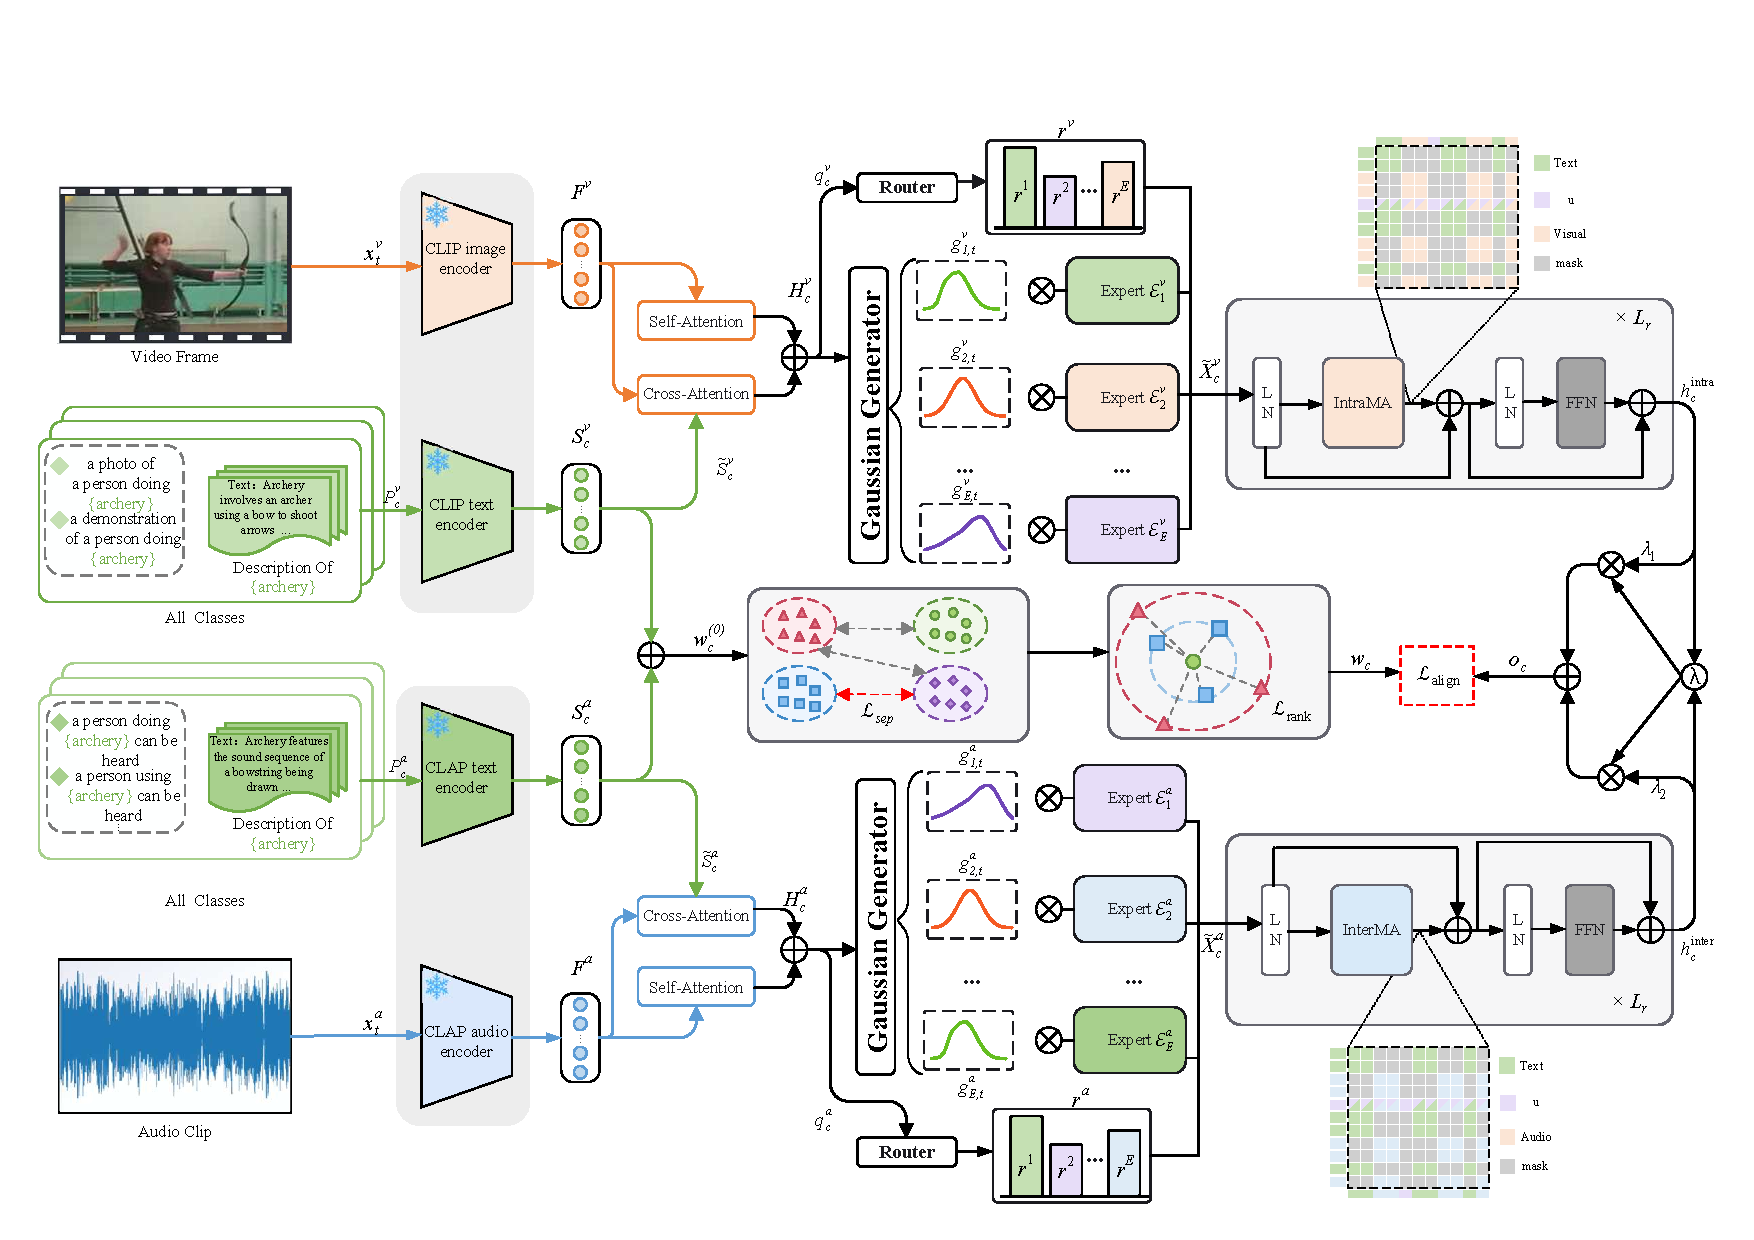
\includegraphics[pagebox=mediabox,width=\textwidth,trim={12bp 11bp 13bp 51bp},clip]{figures/SGTG.pdf}
\caption{Overall architecture of SGTG. An input video is divided into temporally aligned consecutive segments, from which frozen CLIP image and CLAP audio encoders extract visual and audio sequences. In parallel, frozen text encoders transform the candidate class\textquoteright{}s visual and auditory descriptions into description embeddings, and DSPO produces optimized class embeddings that are subsequently fixed. CGTA conditions each modality sequence on its description embeddings and uses the class embedding to query independent visual and audio Gaussian experts with adaptive routing. Continuous weighting and aggregation produce enhanced sequences and direct audio-visual evidence. DMIF then models temporal relationships through intra-modal and inter-modal encoder branches and applies a three-way dynamic Softmax gate conditioned on the direct evidence and candidate class. Finally, a projection network maps the fused representation to a class-conditioned embedding.}
\label{fig:architecture}
\end{figure*}
